\documentclass[12pt,a4paper]{article}

%%%%%%%%%%%%%%%%%%%%%%%%%%%%%%%%%%%%%%%%%%%%%%%%%%%%%%%%%%%%%%%%%%%%%%%%%%%%
%%%%%%%%%%%%%%%%%%%%%%%%%%%%%%%%%% Packages %%%%%%%%%%%%%%%%%%%%%%%%%%%%%%%%
%%%%%%%%%%%%%%%%%%%%%%%%%%%%%%%%%%%%%%%%%%%%%%%%%%%%%%%%%%%%%%%%%%%%%%%%%%%%

% File directory tree
\usepackage{dirtree}
% Verbatim code / psuedocode styling
\usepackage{etoolbox}
% Graphic (images) styling
\usepackage{graphicx}
% For URL hyperlinks (including in references.bib)
\usepackage{hyperref}
% For musical notation
\usepackage{harmony}
% BibTex styling
\usepackage{natbib}

%%%%%%%%%%%%%%%%%%%%%%%%%%%%%%%%%%%%%%%%%%%%%%%%%%%%%%%%%%%%%%%%%%%%%%%%%%%%
%%%%%%%%%%%%%%%%%%%%%%%%%%%%%%%%%% Commands %%%%%%%%%%%%%%%%%%%%%%%%%%%%%%%%
%%%%%%%%%%%%%%%%%%%%%%%%%%%%%%%%%%%%%%%%%%%%%%%%%%%%%%%%%%%%%%%%%%%%%%%%%%%%

% For monospacing (for package names, variable names, etc.)
\newcommand{\code}{\texttt}

% Better inline directory listings (slightly gray)
\usepackage{xcolor}
\definecolor{light-gray}{gray}{0.95}
\newcommand{\lightcode}[1]{\colorbox{light-gray}{\texttt{#1}}}

% Custom command so we write 4-4 time.
\newcommand{\setmeter}[2]{\ensuremath{%
  \vcenter{\offinterlineskip
    \halign{\hfil##\hfil\cr
            $\scriptstyle#1$\cr
            \noalign{\vskip1pt}
            $\scriptstyle#2$\cr}
  }}%
}

%%%%%%%%%%%%%%%%%%%%%%%%%%%%%%%%%%%%%%%%%%%%%%%%%%%%%%%%%%%%%%%%%%%%%%%%%%%%
%%%%%%%%%%%%%%%%%%%%%%%%%%%%%% Page dimensions %%%%%%%%%%%%%%%%%%%%%%%%%%%%%
%%%%%%%%%%%%%%%%%%%%%%%%%%%%%%  DO NOT CHANGE  %%%%%%%%%%%%%%%%%%%%%%%%%%%%%
%%%%%%%%%%%%%%%%%%%%%%%%%%%%%%%%%%%%%%%%%%%%%%%%%%%%%%%%%%%%%%%%%%%%%%%%%%%%

\textheight=247mm
\textwidth=160mm
\topmargin=-7mm
\oddsidemargin=-2mm
\evensidemargin=-8mm
\parindent 10pt

%%%%%%%%%%%%%%%%%%%%%%%%%%%%%%%%%%%%%%%%%%%%%%%%%%%%%%%%%%%%%%%%%%%%%%%%%%%%%
%%%%%%%%%%%%%%%%%%%%%%%%%%%%% Start of document %%%%%%%%%%%%%%%%%%%%%%%%%%%%%
%%%%%%%%%%%%%%%%%%%%%%%%%%%%%%%%%%%%%%%%%%%%%%%%%%%%%%%%%%%%%%%%%%%%%%%%%%%%%

\begin{document}
\pagestyle{plain}
\pagenumbering{arabic}

%%%%%%%%%%%%%%%%%%%%%%%%%%%%%%%%%%%%%%%%%%%%%%%%%%%%%%%%%%%%%%%%%%%%%%%%%%%%%
%%%%%%%%%%%%%%%%%%%%%%%%%%%%% Title of proposal %%%%%%%%%%%%%%%%%%%%%%%%%%%%%
%%%%%%%%%%%%%%%%%%%%%%%%%%%%%%%%%%%%%%%%%%%%%%%%%%%%%%%%%%%%%%%%%%%%%%%%%%%%%

\begin{center}
{\LARGE{\bf
%%
%% TITLE
{{Procedural Soundscape}}
%%
%%
}}
\end{center}
\bigskip

%% Principal Investigator (PI) initial(s) and family name %%
\centerline{\bf{Claire Goeckner-Wald \& Amy Xiong}}

\bigskip

% Type a concise abstract of your proposal here (optional).
\tableofcontents

%%%%%%%%%%%%%%%%%%%%%%%%%%%%%%%%%%%%%%%%%%%%%%%%%%%%%%%%%%%%%%%%%%%%%%%%%%%%%%%%%%%%%%%%%
%%%%%%%%%%%%%%%%%%%%%%%%%%%%%%%%%%%%% Introduction %%%%%%%%%%%%%%%%%%%%%%%%%%%%%%%%%%%%%%
%%%%%%%%%%%%%%%%%%%%%%%%%%%%%%%%%%%%%%%%%%%%%%%%%%%%%%%%%%%%%%%%%%%%%%%%%%%%%%%%%%%%%%%%%
\pagebreak
\section{Executive Summary}

\textbf{A short overview of your project idea, why it is interesting and what you would like to learn from it.}

We built a website with a procedural-generated soundscape inspired by `\href{https://www.youtube.com/watch?v=K2Q6YO3Ez44}{coffeehouse jazz}'. While we did not integrate the soundscape with live variables, we did integrate it with a synesthetic background image. It would not be terribly difficult to integrate the soundscape with live variables at this point, but we chose not to due to time constraints. (Amy: discuss musical `palette' here.) We chose to use \lightcode{tonejs-instruments} because it integrated open-source \code{WAV}-format files from real instruments with \lightcode{Tone.js} \cite{tonejs-instruments}. We tested the final product in both Mozilla Firefox Quantum 63.0 and Google Chrome 70.0. Rather than using Google App Engine, or similar, we simply hosted the website for free on Claire's personal GitHub site, \href{https://cgoecknerwald.github.io/procedural-soundscape}{cgoecknerwald.github.io/procedural-soundscape}. This greatly simplified the workflow, as we could easily push HTML/CS/JS to the GitHub repository, and it would then be immediately updated online with no extra work.

\subsection{Description}
\textbf{Brief description of features}

The entire codebase (and the original \code{LaTeX} files for this very report) can be found on Claire's GitHub repository: \href{https://github.com/cgoecknerwald/procedural-soundscape}{github.com/cgoecknerwald/procedural-soundscape}. The web application is live at \href{https://cgoecknerwald.github.io/procedural-soundscape/}{cgoecknerwald.github.io/procedural-soundscape/}.

\begin{itemize}
	\item A web application
	\item A procedural soundscape
	\item A visual landscape
\end{itemize}

\subsection{Technical Requirements}
\textbf{Audio requirements (and probably also requirements necessary to run the files)}

\begin{itemize}
	\item Browser: Firefox Quantum 63.0 and above, or Google Chrome 70.0 and above.
	\item User input: Interaction with web browser via cursor.
	\item User output: Any functioning speakers will do.
\end{itemize}

\subsection{Technical Challenges}
We did not test at all on Internet Explorer, only Firefox and Chrome. We had issues with \lightcode{Tone.js}.

\subsection{Licensing}
We chose to license our repository with the MIT License.


%%%%%%%%%%%%%%%%%%%%%%%%%%%%%%%%%%%%%%%%%%%%%%%%%%%%%%%%%%%%%%%%%%%%%%%%%%%%%%%%%%%%%%%%%
\pagebreak
\section{Technical Design}
\textbf{In-depth technical design and reasons for choosing this design}

\subsection{Sound Design Tool Discussion}
We've decided to use \lightcode{Tone.js} instead of \lightcode{Audiosynth.js} by Keith William Horwood. We also chose \lightcode{Tone.js} over \lightcode{SuperCollider}, \lightcode{Flocking.js}, \lightcode{PureData}, because of web integration ease. \lightcode{Flocking.js} also had web integration but a smaller online community and seemed less robust and less abstracted. \lightcode{Audiosynth.js} did not have looping technologies. We briefly considered integrating our whole product with \lightcode{Audiosynth.js} but it proved to be too difficult.

\subsubsection{PureData}
\lightcode{PureData} was far too low-level (and therefore tedious and slow) for our plans.

\begin{quote}
Pure Data is an open source visual programming environment that runs on anything from personal computers to embedded devices (ie Raspberry Pi) and smartphones (via libpd, DroidParty (Android), and PdParty (iOS). It is a major branch of the family of patcher programming languages known as Max (Max/FTS, ISPW Max, Max/MSP, etc), originally developed by Miller Puckette at IRCAM.

Pd enables musicians, visual artists, performers, researchers, and developers to create software graphically without writing lines of code. Pd can be used to process and generate sound, video, 2D/3D graphics, and interface sensors, input devices, and MIDI. Pd can easily work over local and remote networks to integrate wearable technology, motor systems, lighting rigs, and other equipment. It is suitable for learning basic multimedia processing and visual programming methods as well as for realizing complex systems for large-scale projects.

Algorithmic functions are represented in Pd by visual boxes called objects placed within a patching window called a canvas. Data flow between objects are achieved through visual connections called patch cords. Each object performs a specific task, which can vary in complexity from very low-level mathematical operations to complicated audio or video functions such as reverberation, FFT transformations, or video decoding. Objects include core Pd vanilla objects, external objects or externals (Pd objects compiled from C or C++), and abstractions (Pd patches loaded as objects). \cite{puredata}
\end{quote}

\subsubsection{SuperCollider}
SuperCollider seemed okay at first, but we could not see an easy way to integrate it with HTML/JS/CSS (knowing that we wanted to build a web application).

\begin{quote}
SuperCollider is a platform for audio synthesis and algorithmic composition, used by musicians, artists, and researchers working with sound. It is free and open source software available for Windows, macOS, and Linux. \cite{supercollider}
\end{quote}

\subsubsection{Flocking.js}
\lightcode{Flocking.js} was a strong contender for our choice of sound design technology.

\begin{quote}
Flocking is a JavaScript audio synthesis framework designed for artists and musicians who are building creative and experimental Web-based sound projects. It runs in Firefox, Chrome, Safari, Edge, and Node.js on Mac OS X, Windows, Linux, iOS, and Android.

Flocking is different. Its goal is to promote a uniquely community-minded approach to instrument design and composition. In Flocking, unit generators and synths are specified declaratively as JSON, making it easy to save, share, and manipulate your synthesis algorithms. Send your synths via Ajax, save them for later using HTML5 local data storage, or algorithmically produce new instruments on the fly.

Because it's just JSON, every instrument you build using Flocking can be easily modified and extended by others without forcing them to fork or cut and paste your code. This declarative approach will also help make it easier to create new authoring, performance, metaprogramming, and social tools on top of Flocking.

Flocking was inspired by the SuperCollider desktop synthesis environment. If you're familiar with SuperCollider, you'll feel at home with Flocking. \cite{flocking}
\end{quote}

\subsubsection{Audiosynth.js}

\begin{quote}
Dynamic waveform audio synthesizer, written in Javascript. Generate musical notes dynamically and play them in your browser using the HTML5 Audio Element. No static files required. (Besides the source, of course!) \cite{audiosynth}
\end{quote}


\subsubsection{Tone.js}
In the end, we chose \lightcode{Tone.js} out of all three Javascript sound design frameworks for its robust online community (and therefore support).

\begin{quote}
Tone.js is a Web Audio framework for creating interactive music in the browser. The architecture of Tone.js aims to be familiar to both musicians and audio programmers looking to create web-based audio applications. On the high-level, Tone offers common DAW (digital audio workstation) features like a global transport for scheduling events and prebuilt synths and effects. For signal-processing programmers (coming from languages like Max/MSP), Tone provides a wealth of high performance, low latency building blocks and DSP modules to build your own synthesizers, effects, and complex control signals. \cite{tonejs}
\end{quote}

%%%%%%%%%%%%%%%%%%%%%%%%%%%%%%%%%%%%%%%%%%%%%%%%%%%%%%%%%%%%%%%%%%%%%%%%%%%%%%%%%%%%%%%%%
\subsection{Technological Review}
\textbf{Discuss relevant github repos and projects and articles}
We looked at Karplus-Strong String Synthesis but determined it was only relevant if we used \lightcode{Audiosynth.js} \cite{karplus-strong}.

\subsubsection{Tambien's Tone.js}
For the reasons discussed in `2. Sound Design Tool Discussion' above, we ultimately chose \lightcode{Tone.js} as our main sound design package.

\subsubsection{Nbrosowsky's tonejs-instruments}
The package \lightcode{tonejs-instruments} was instrumental (haha) in our final project. It features all soundclips in \code{WAV}, \code{MP3}, and \code{OGG} formats.

\subsubsection{Wheelibin's synaesthesia}
We modified his drum kit and synths. We based our \code{assets/jschords.js} and \code{assets/js/rhythms.js} off of \lightcode{synaesthesia}.

\subsubsection{Tambien's jazz.computer}
We got mostly drums synths and pads from \code{tambien} (Yotam Mann, creator of \lightcode{Tone.js})'s \href{http://jazz.computer/}{\lightcode{jazz.computer}} (works best in Chrome or Safari). \code{Tambien}'s \href{http://jazz.computer/}{\lightcode{jazz.computer}} but they had a very strange music set-up with interpolation and mediators between synths. We attempted to replicate by playing mulitple synths simulataneously but the resulting 'piano' was very tinny and sounded like Scottish bagpipes.


%%%%%%%%%%%%%%%%%%%%%%%%%%%%%%%%%%%%%%%%%%%%%%%%%%%%%%%%%%%%%%%%%%%%%%%%%%%%%%%%%%%%%%%%%
\subsection{Musical Review}

The first challenge was in getting \lightcode{Tone.js} to produce random music that would play forever.

\subsubsection{Scheduling}
\lightcode{Tone.js}'s has a scheduling system for producing music. \lightcode{Tone.js} had scheduling components that allowed you to play a series of notes in a row (e.g. \lightcode{Tone.Part}).

\lightcode{Tone.js} can only repeat in regular intervals. It could not, for example, calculate the amount of time a section of music would take, then automatically repeat after that section was finished. This meant we had to make each randomly-generated section of music be of the same length, in order for them to fit together without breaks in the music. We thus decided to generate music one measure at a time.

\lightcode{Tone.js} allows you to have multiple notes playing at the same time. Thus, you must specify both the duration of the note and when it should be played, not just one or the other. We had to thus separately track the time elapsed as we randomly generated our notes, in order to be able to know when to schedule the next note.

\lightcode{triggerAttackRelease(note, duration, time)}

\subsubsection{Rhythm}

For random rhythm patterns, we used a set of 8 rhythms patterns \cite{common-rhythms}:

% if we can use package harmony, commands are in comments
\begin{center}
\begin{tabular}{ l r }
whole & \Ganz \\
half half & \Halb \Halb \\
dotted-half quarter & \Halb\Pu \Vier \\
quarter dotted-half & \Vier \Halb\Pu \\
half quarter quarter & \Halb \Vier \Vier \\
quarter half quarter & \Vier \Halb \Vier \\
quarter quarter half & \Vier \Vier \Halb \\
quarter quarter quarter quarter & \Vier \Vier \Vier \Vier \\
\end{tabular}
\end{center}

All rhythm constants are stored in \lightcode{assets/js/rhythms.js}.

Note that each of these rhythms take up exactly one measure (in \setmeter{4}{4} time).
We then augmented this set by using the same patterns with shorter notes. We halved all the note lengths to get an equivalent set of rhythm patterns that take up half a measure, and then halved the lengths again to get another set that take up one quarter note.

We generate music one measure at a time, but within each measure, we generate the measure by connecting together these rhythm patterns. Since some of the patterns are shorter than a measure (the length of either one quarter note or one half note), we must be sure to generate the appropriate number of rhythm-segments, of the appropriate length, to exactly equal one measure of music.

For example, we might generate a measure of music by first generating four sixteenth-notes (a one-quarter-note rhythm pattern), then one half-note (a one-half-note rhythm pattern), then finally two eighth-notes (a one-quarter-note rhythm pattern again). We cannot, however, generate first four sixteenth-notes, then four quarter-notes, as that will last longer than one measure. We also cannot generate four sixteenth-notes, then one half-note, then stop, since that will last shorter than one measure.

We have the function \lightcode{createMeasure(maxLength, offset)} to create notes with a single rhythm pattern. The parameters specify the maximum length of music to generate (1-4 quarter notes) and the offset into the measure the notes should start at (0-3 quarter notes in). The function first randomly decides what length of music to generate (1, 2, or 4 quarter notes of music) that falls within the maximum length. It randomly picks one of the 8 possible rhythms. The shorter rhythms (half-note-length or quarter-note-length) are obtained by dividing the note lengths according to whether it's generating 1, 2, or 4 quarter notes of music.

\subsubsection{Pitch Generation}

Pitches are also randomly generated. When the website is first loaded, it randomly picks a tonic note and a scale type to build a scale (e.g. C Major, A-flat Minor, D-sharp Dorian). Note pitches are chosen only from this scale.

%%%%%%%%%%%%%%%%%%%%%%%%%%%%%%%%%%%%%%%%%%%%%%%%%%%%%%%%%%%%%%%%%%%%%%%%%%%%%%%%%%%%%%%%%
\subsection{User Interface}
We wanted to make our user interface fun without being confusing, or being so difficult to implement that it distracts from the work of sound design. We settled on a semi-transparent paneling design that would allow us to compartmentalize the different functions while showing off a collection of highly-textured backgrounds.

\begin{figure}
\centering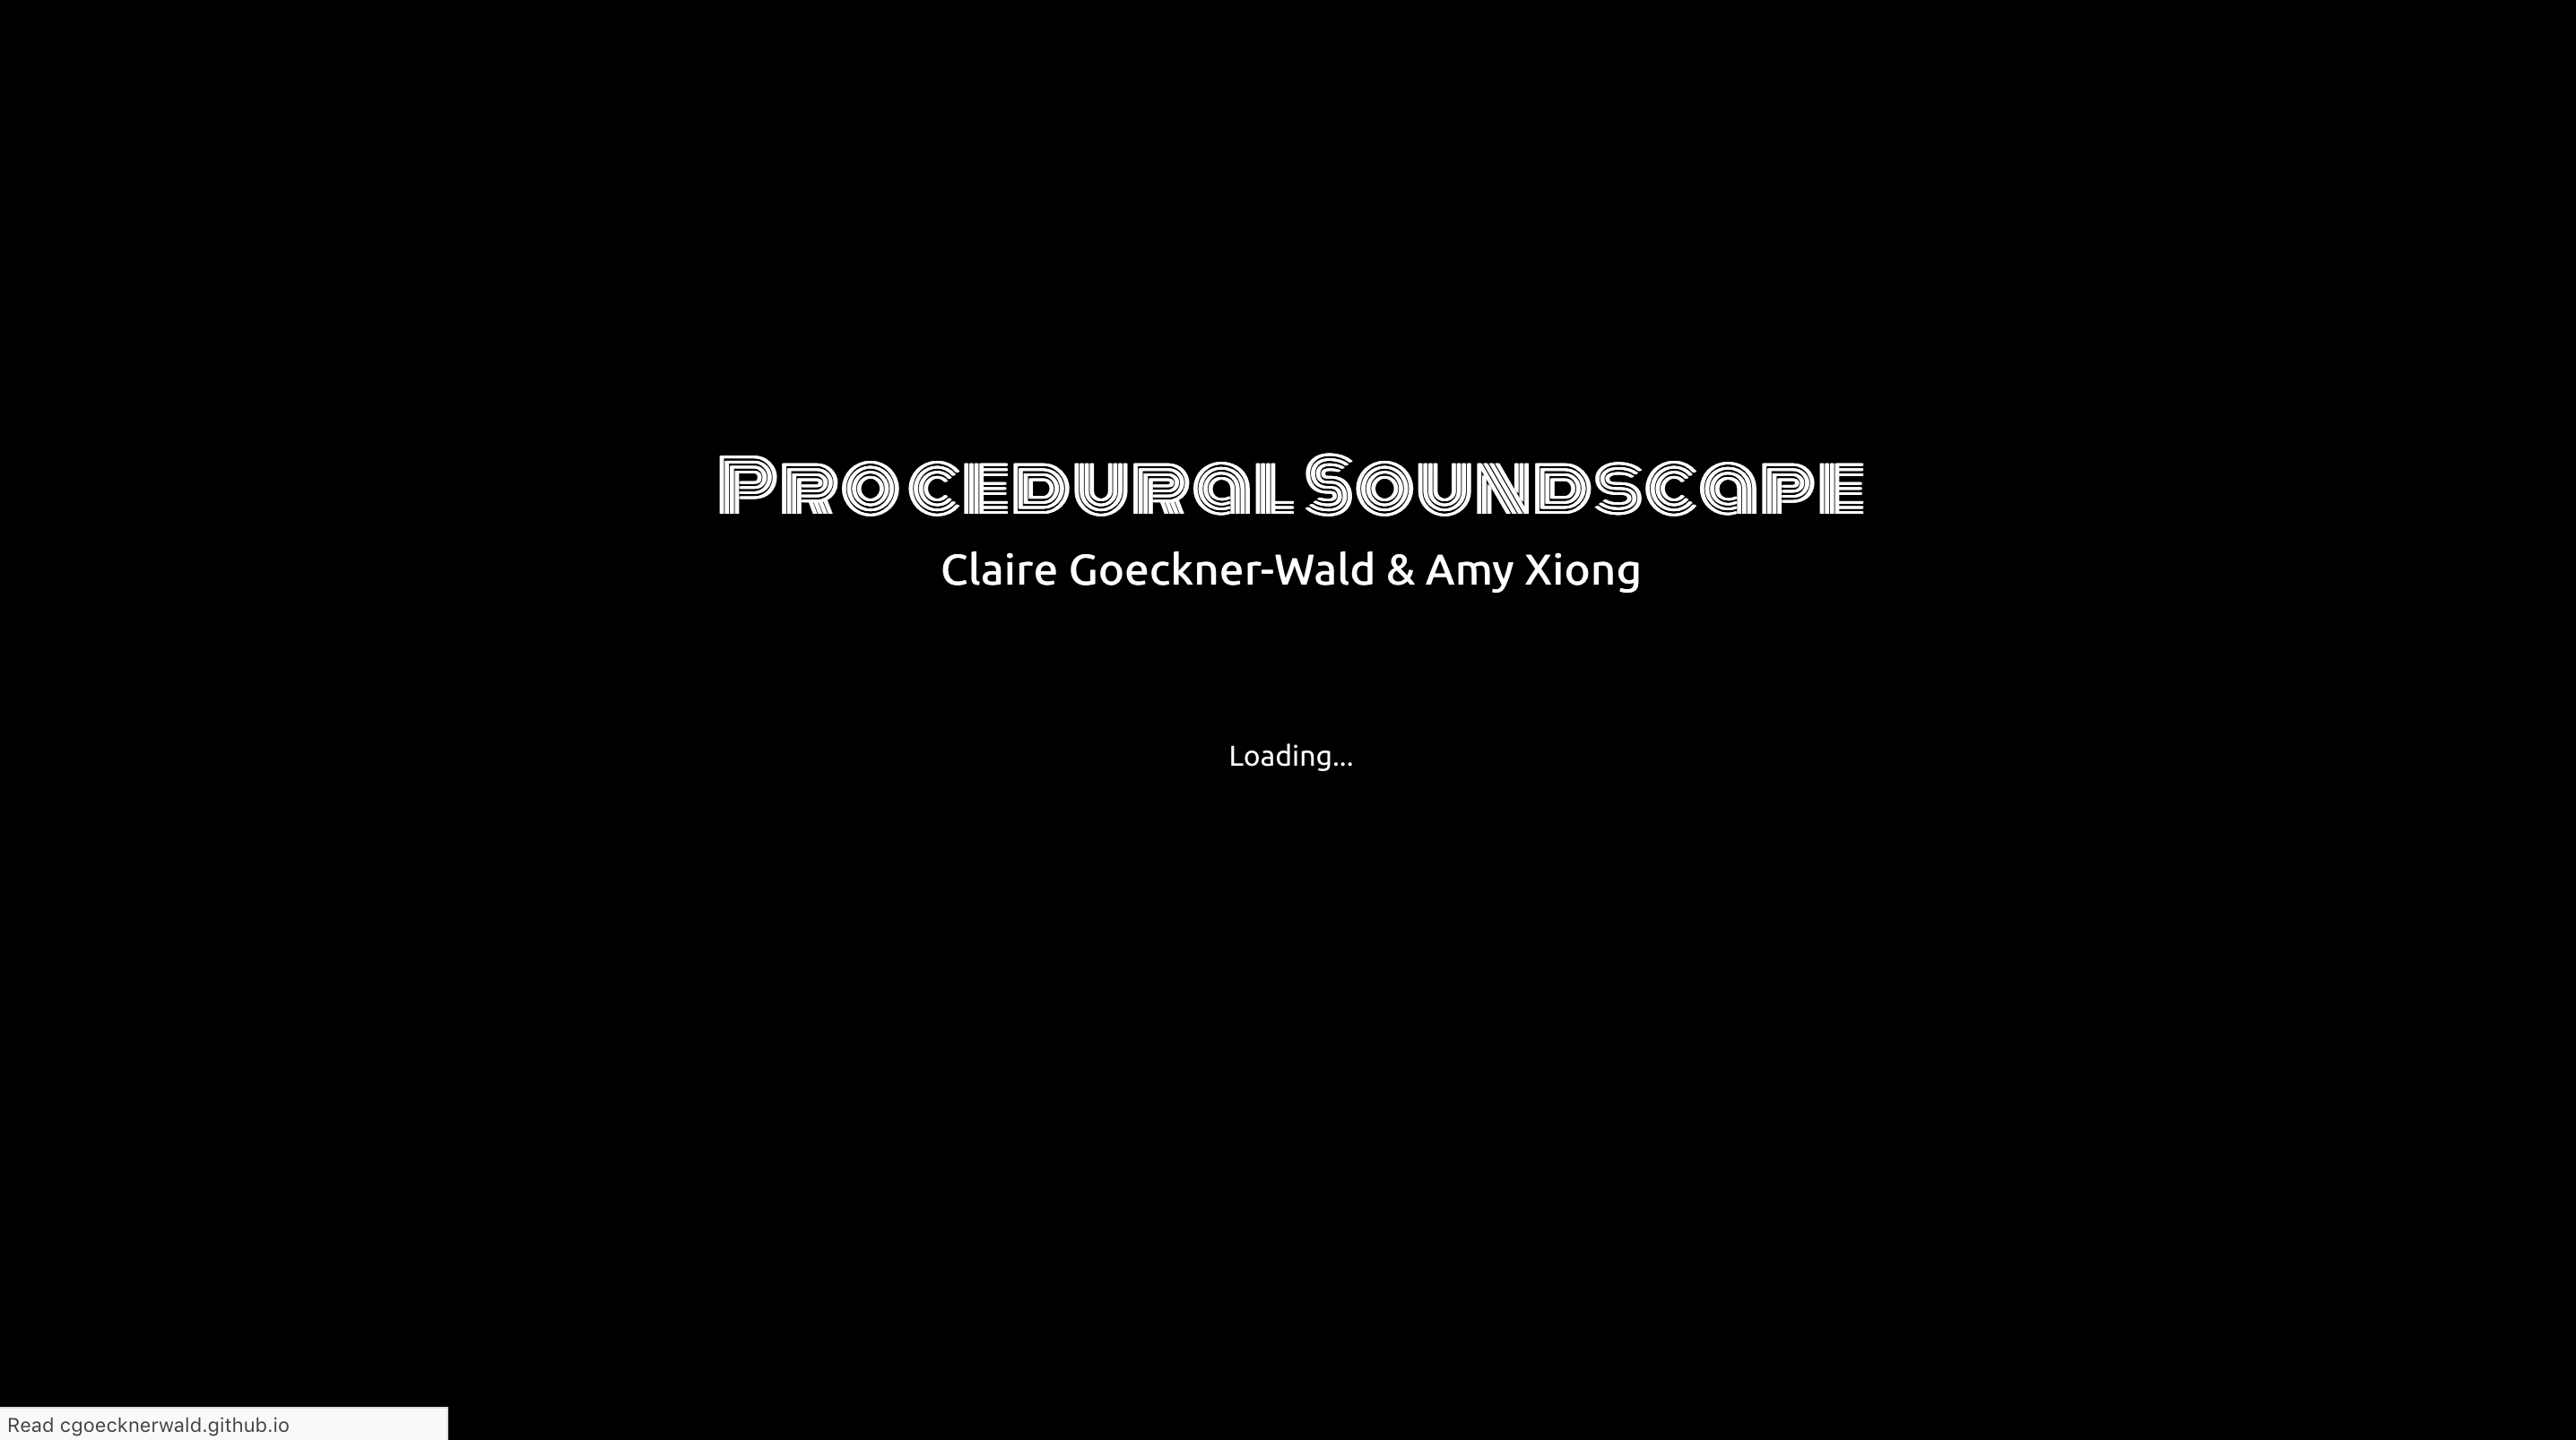
\includegraphics[width=0.8\textwidth]{images/loading.png}
\caption{The loading screen as seen on Firefox Quantum 63.0. During this screen, fonts, and \code{WAV} soundfiles are loading.}
\end{figure}

\begin{figure}
\centering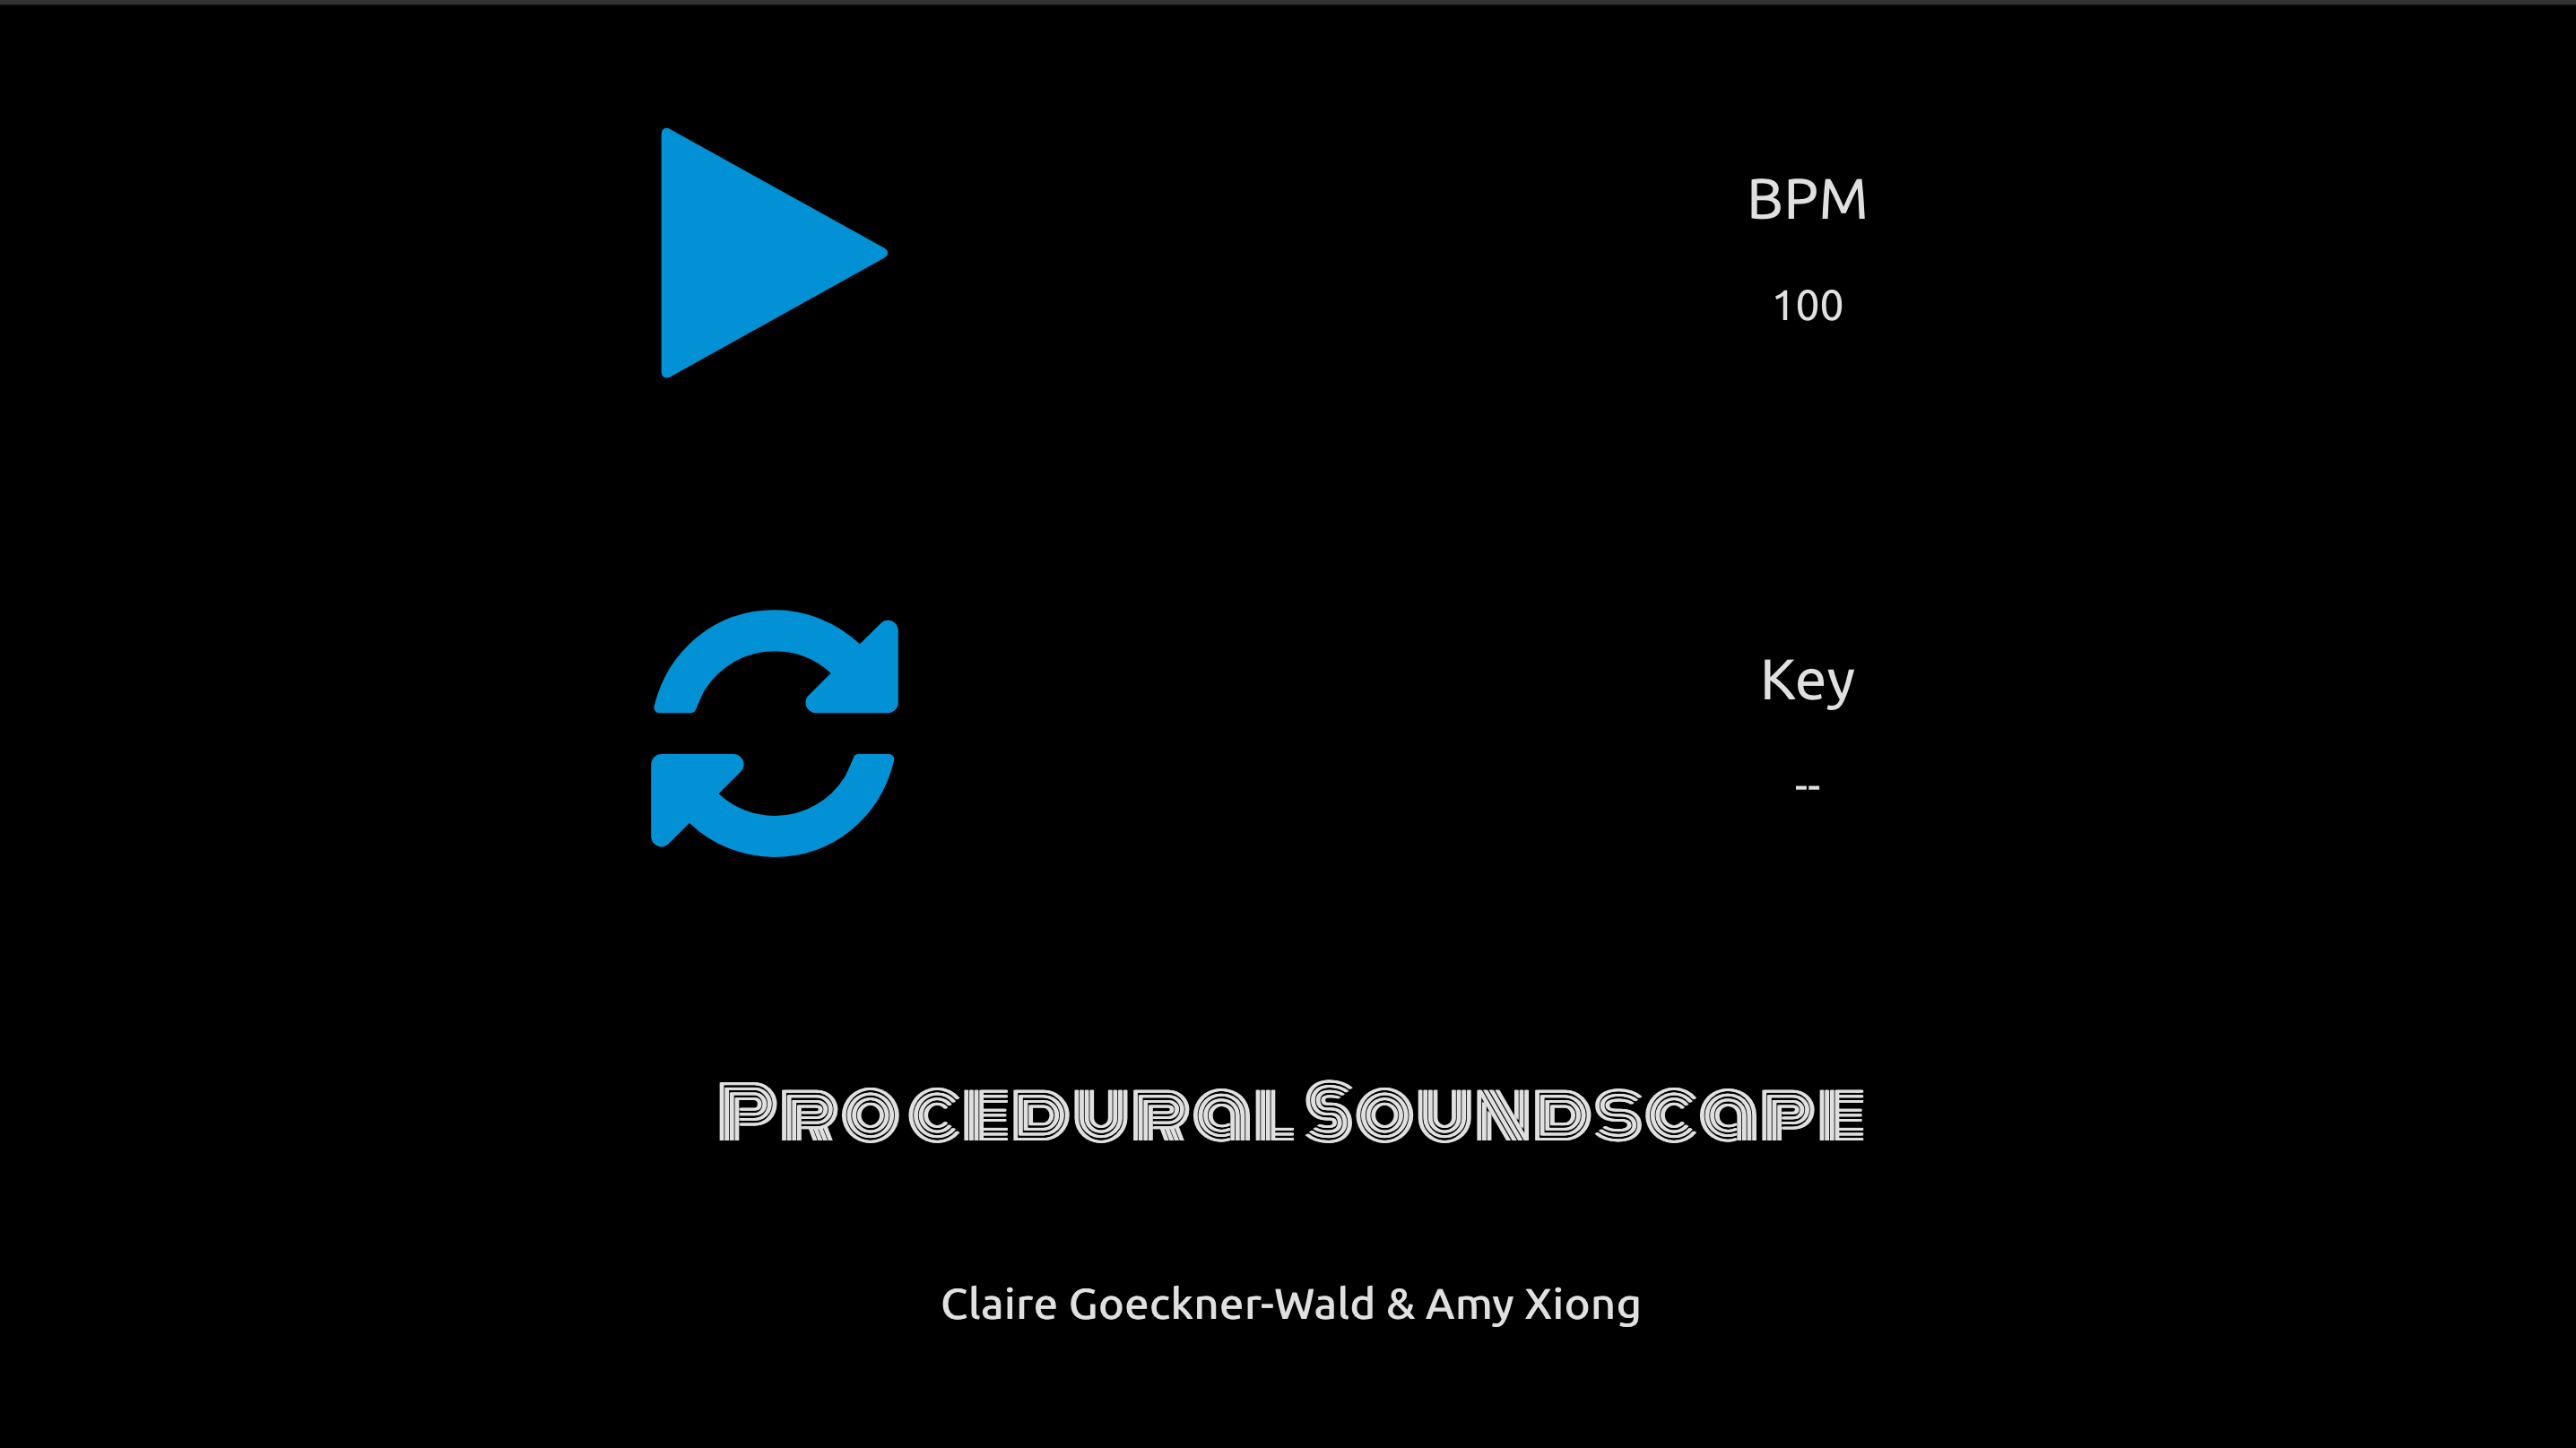
\includegraphics[width=0.8\textwidth]{images/loaded.png}
\caption{The pre-interaction screen as seen on Firefox Quantum 63.0. This screen occurs after loading is finished, but before the user has interacted with the interface. To begin, users can interact with the play/pause button and the reload/refresh button.}
\end{figure}

\begin{figure}
\centering\includegraphics[width=0.8\textwidth]{images/ui.png}
\caption{The post-interaction user interface as seen on Firefox Quantum 63.0. Users can interact with the play/pause button and the reload/refresh button.}
\end{figure}

\subsubsection{Actions}

There are two actions a user make take: toggle play-pause button or toggle refresh button. Toggling the play-pause button functions exactly as expected - if the music is playing, it stops the music. If the music is not playing, it restarts the music exactly where it left off (or, at the beginning, if toggled for the first time). Toggling the refresh button updates the background, BPM, and key. It necessarily restarts the music, as well.

The first time that either the play-pause button or refresh button is toggled, the program initializes a background, BPM, and key. These three qualities are \textit{unlinked}, meaning they change independently of each other. We considered using a \lightcode{constants.json} file to build dependencies between the backgrounds and the type of music. However, given the large variety of backgrounds we wished to use, we found that this functionality would be cumbersome without adding significant value to the project.

The program also features a count-down because we generate notes a full measure in advance (so that we may display them on screen). Without this extrapolative generation, we may encounter an issue with \lightcode{Tone.js} where the first note is not scheduled in advance of being played, causing the first note to be `dropped,' or not played at all.

\subsubsection{Displays}

There are 3 different kinds of dynamic information displays to the user: the notes, the BPM, and the key.

The notes are scheduled a full measure in advance, which allows us to display them on screen. The function \lightcode{emphasizeNote()} uses the index of the currently sounded note to updated the displayed HTML. In this way, the user can visually track the notes (or rests!) as they are sent live to \lightcode{Tone.js}.


\subsubsection{Backgrounds}

The project features approximately 50 unique backgrounds (the number fluctuates when we delete one we don't like). The backgrounds were selected for their flat, textured appeal from \href{https://unsplash.com/about}{Unsplash} \cite{unsplash}. Unsplash was used for its selection of ``Over 550,000 free (\href{https://unsplash.com/license}{do-whatever-you-want}) high-resolution photos brought to you by the world’s most generous community of photographers,'' with a very generous \href{https://unsplash.com/license}{license}.

\begin{figure}
\centering
\includegraphics[width=0.48\textwidth]{images/bg1.png}
\centering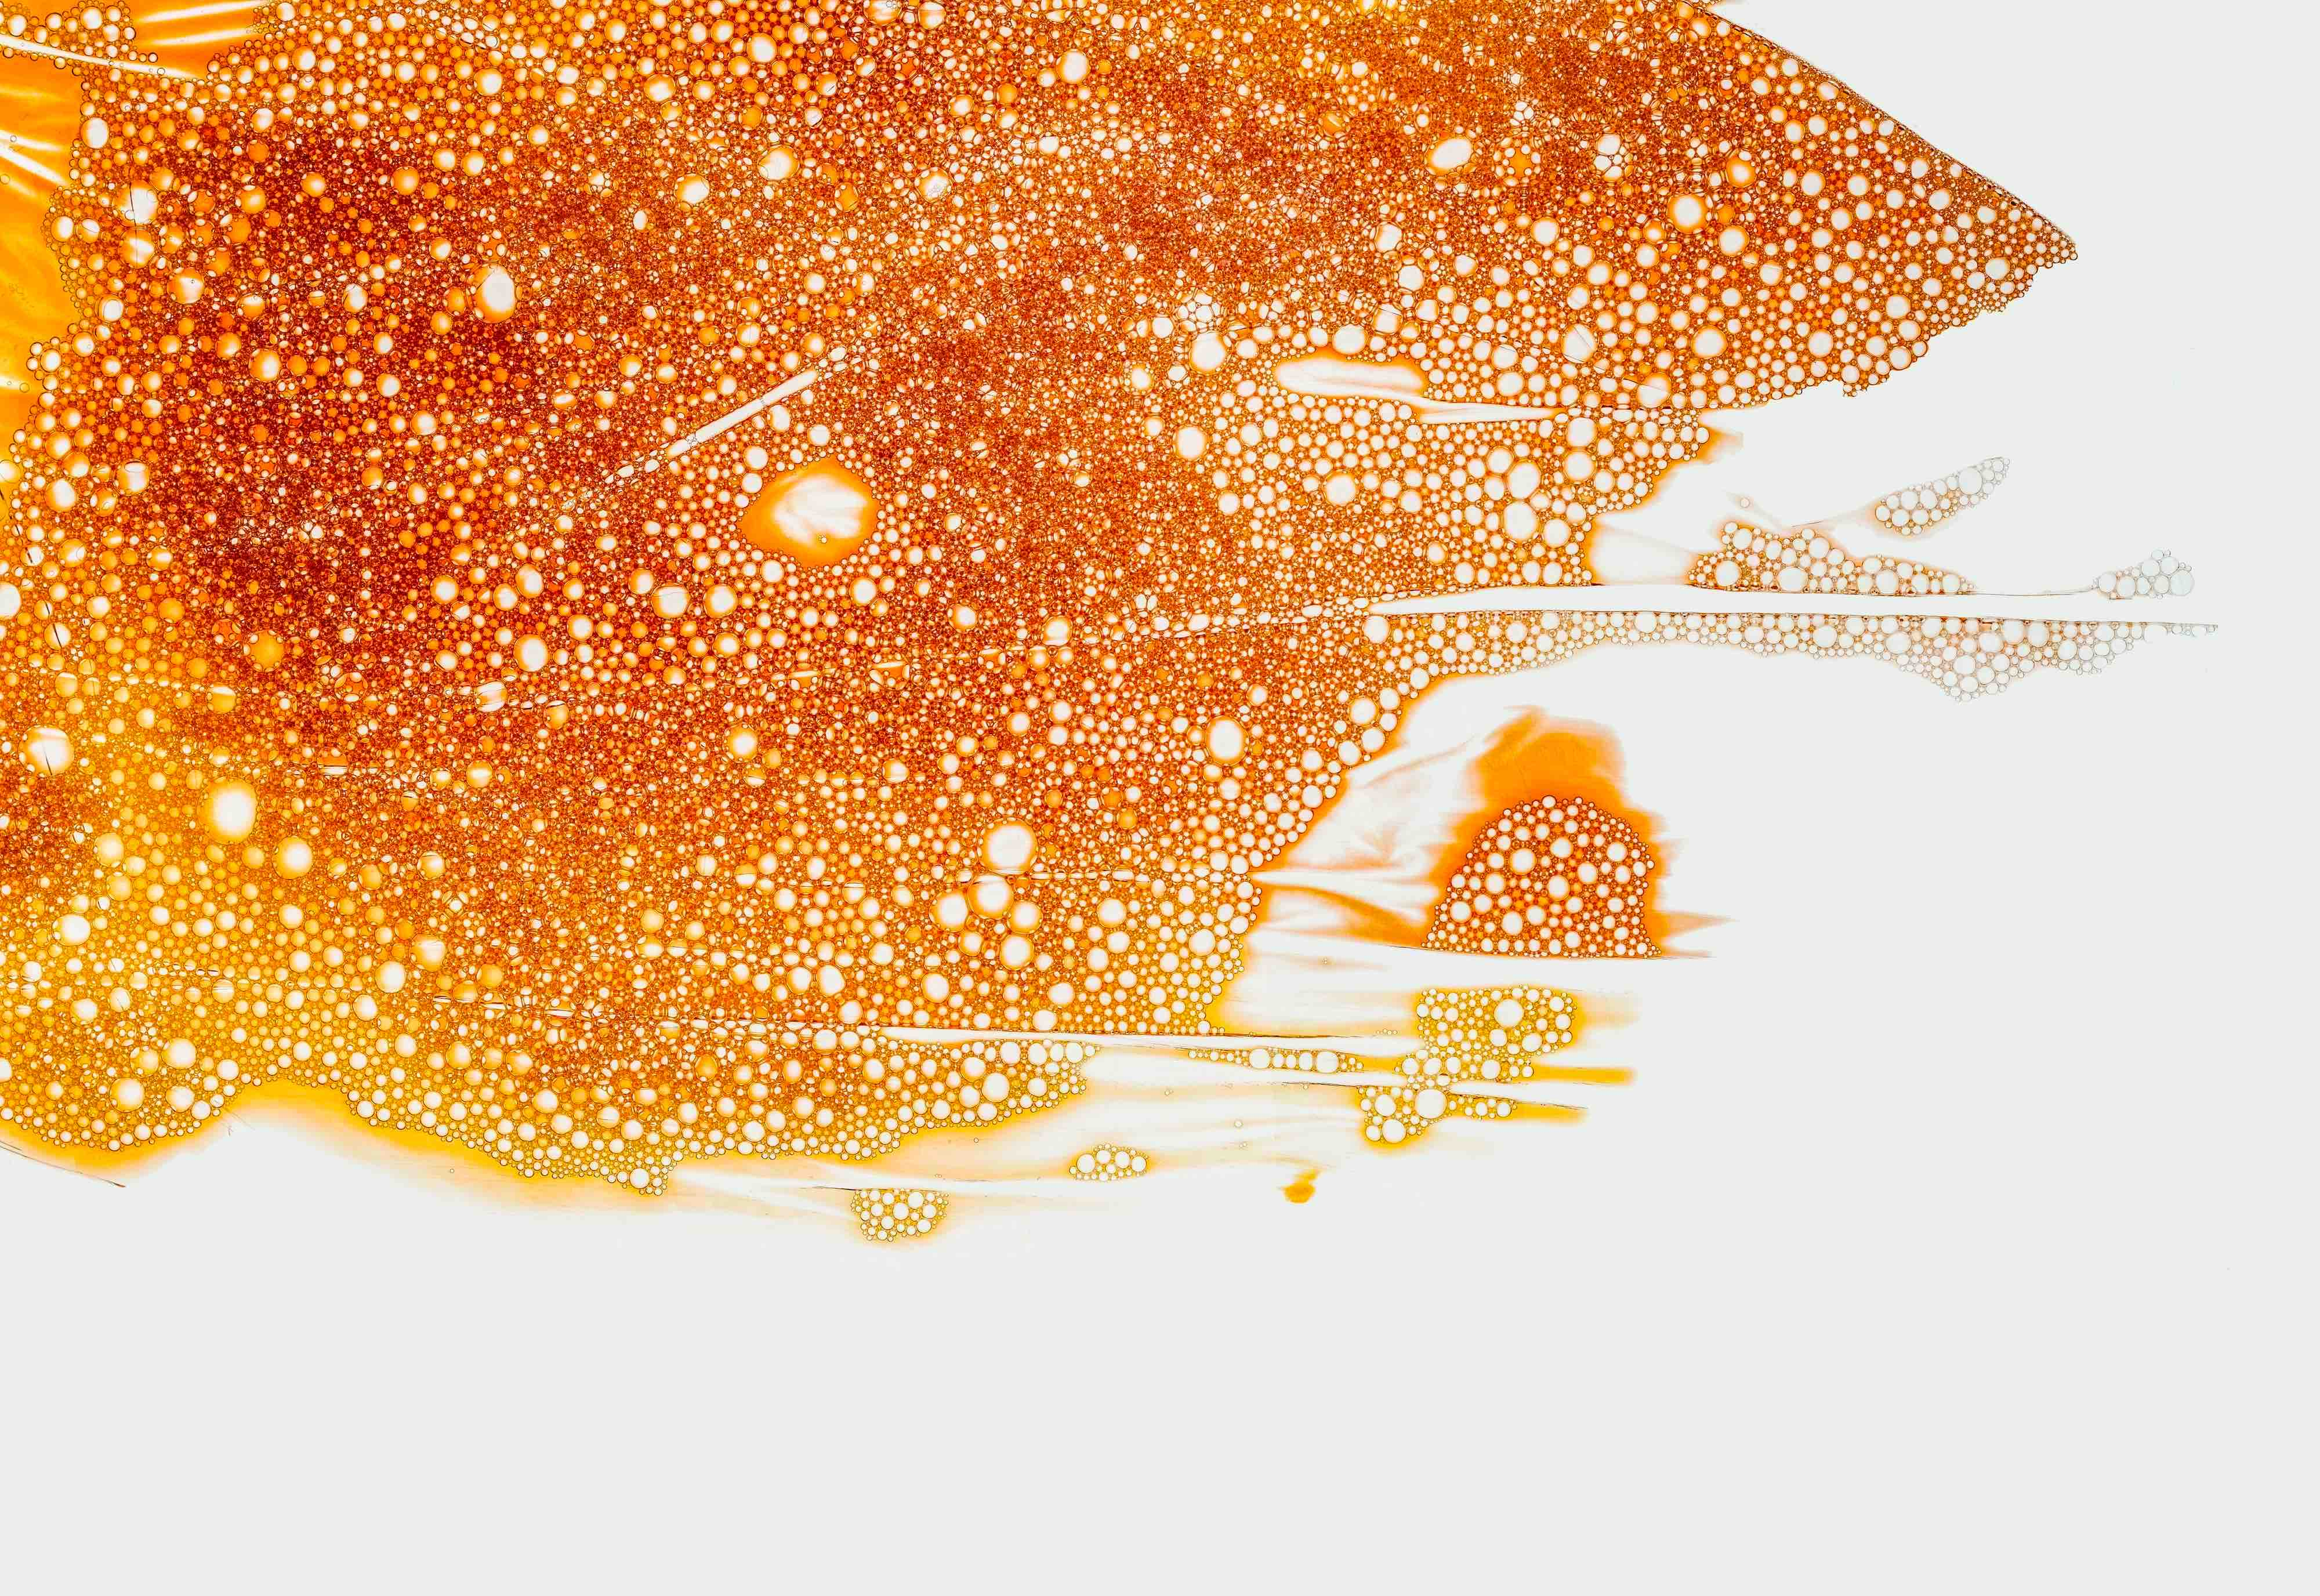
\includegraphics[width=0.48\textwidth]{images/bg2.png}
\centering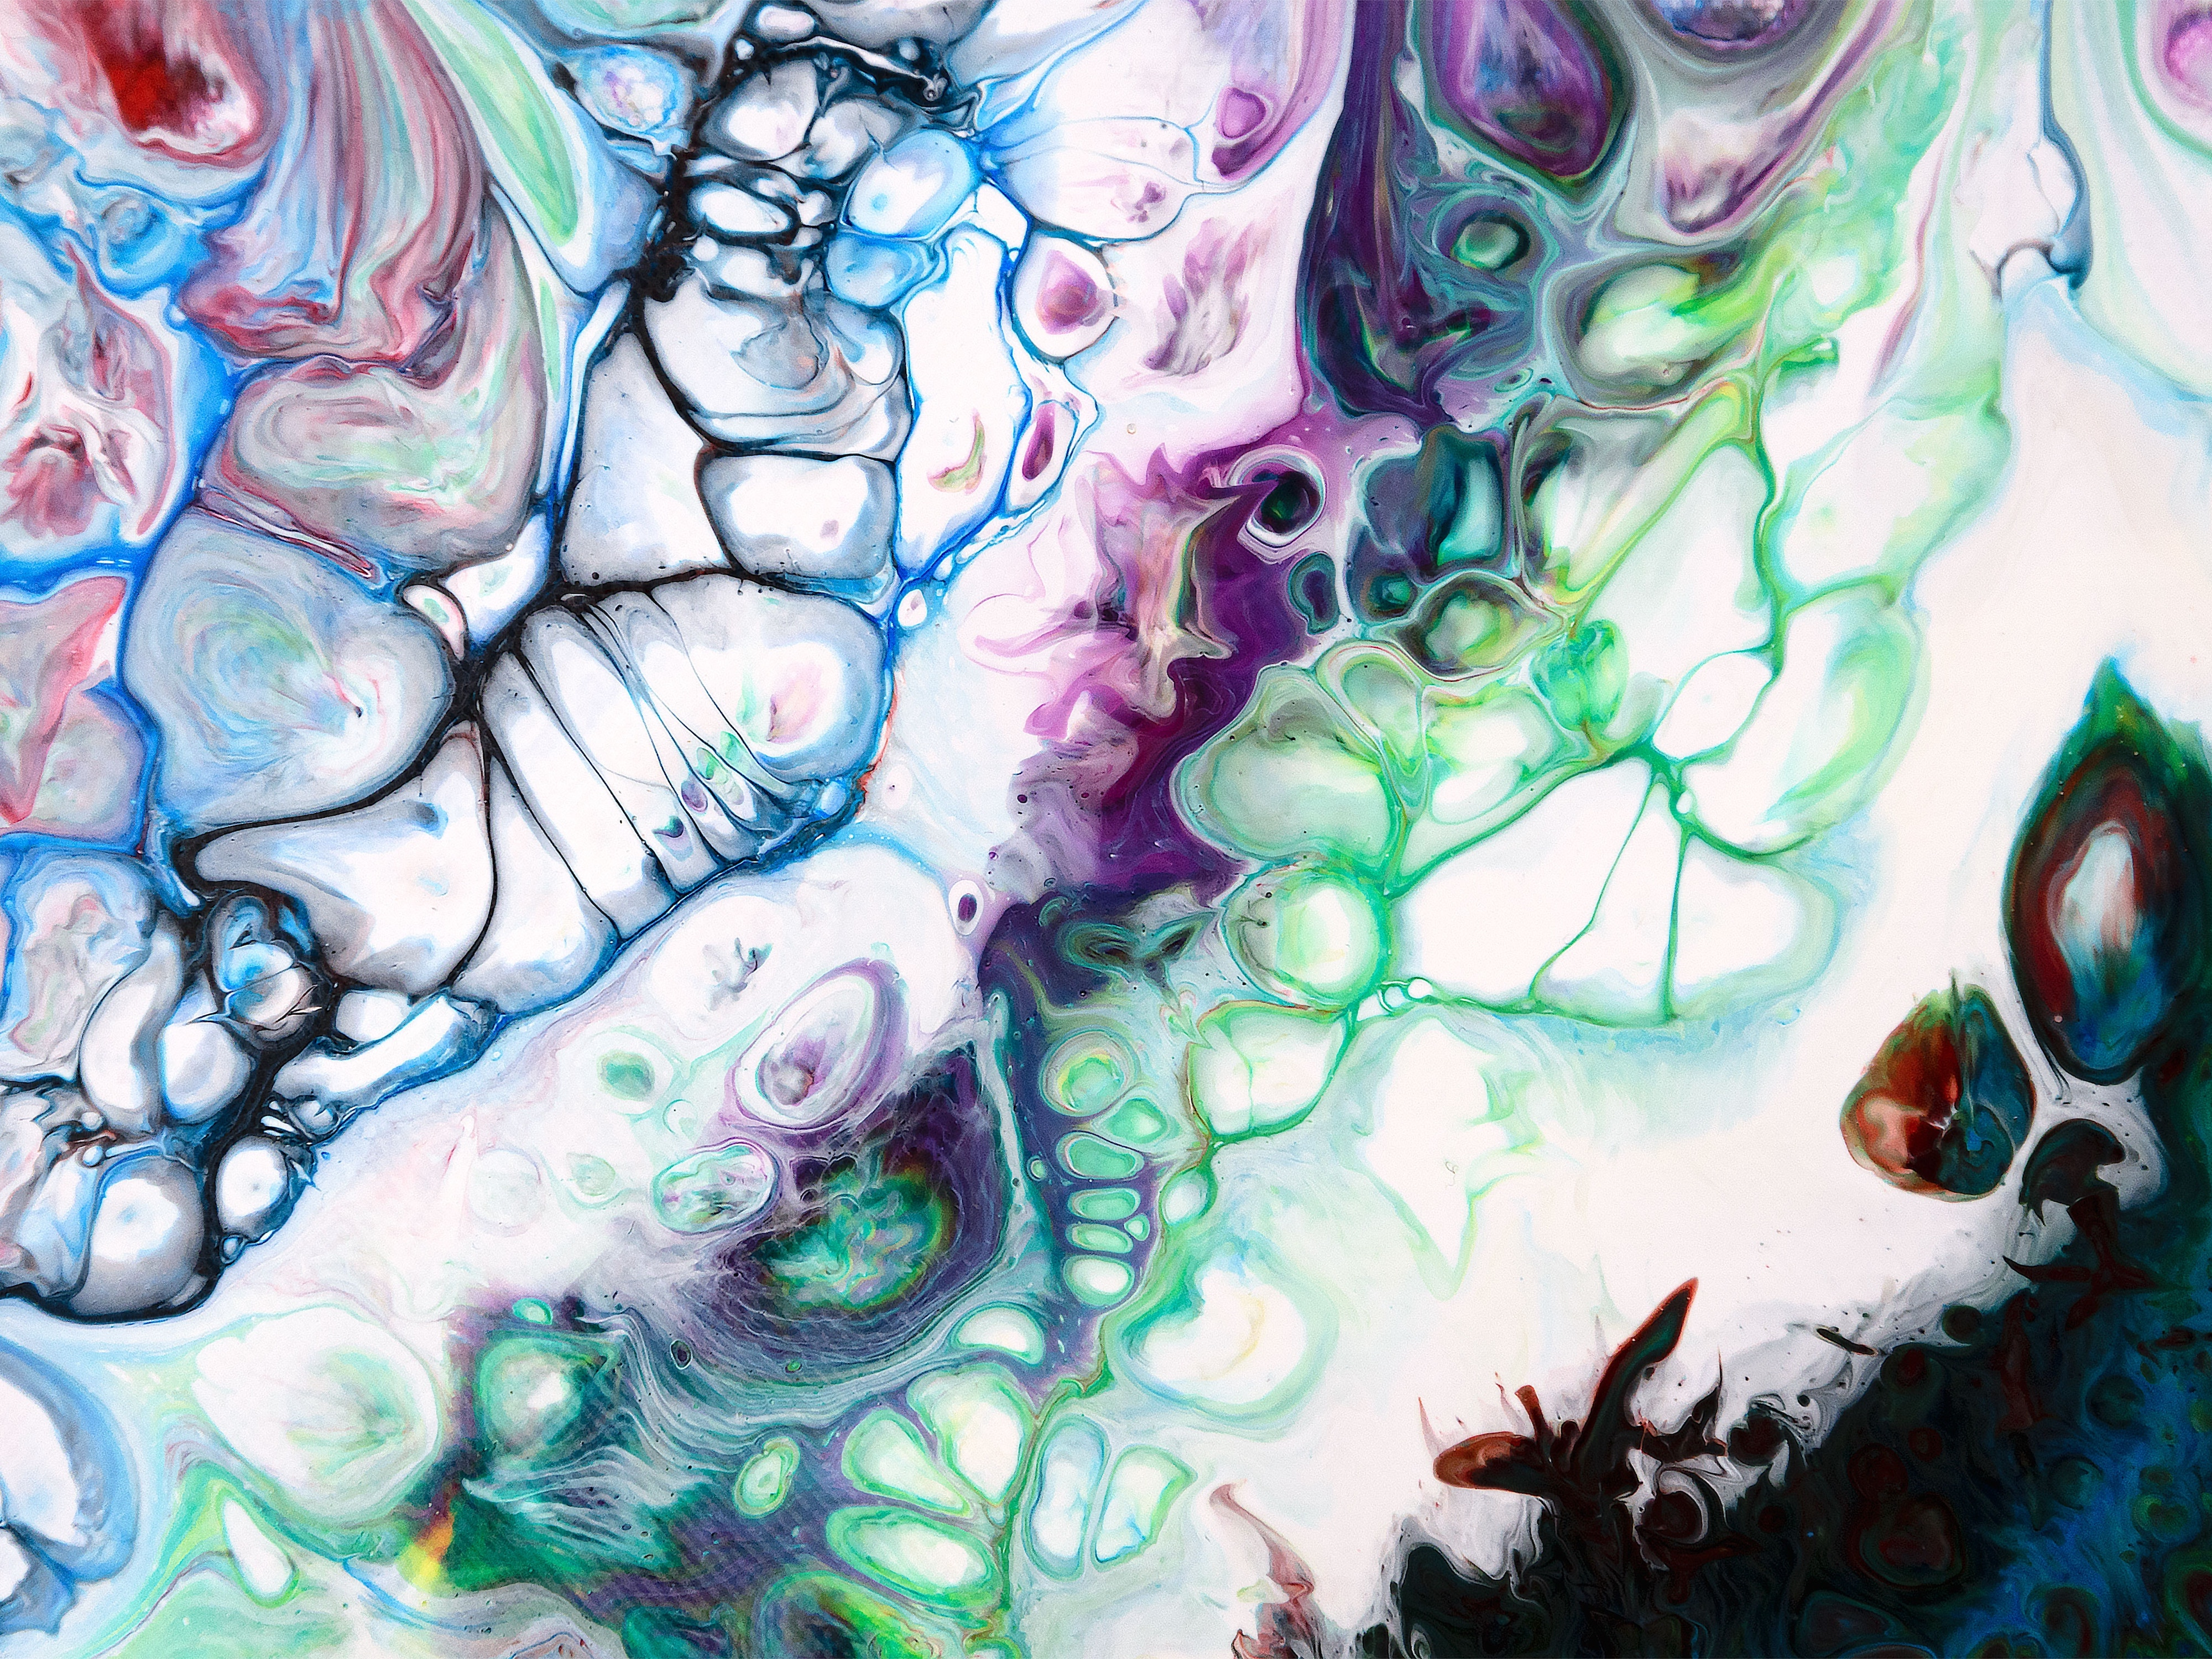
\includegraphics[width=0.48\textwidth]{images/bg3.png}
\centering
\includegraphics[width=0.48\textwidth]{images/bg4.png}
\caption{Various backgrounds.}
\end{figure}


%%%%%%%%%%%%%%%%%%%%%%%%%%%%%%%%%%%%%%%%%%%%%%%%%%%%%%%%%%%%%%%%%%%%%%%%%%%%%%%%%%%%%%%%%
% Must use \clearpage instead of \newpage or \pagebreak, to clear figure environs
\clearpage
\subsection{File Directory Structure}

\dirtree{%
.1 procedural-soundscape.
.2 assets.
.3 backgrounds.
.4 bg0.jpg.
.4 bg1.jpg.
.4 \dots.
.4 bgN.jpg.
.3 css.
.4 main.css.
.3 js.
.4 chords.js.
.4 constants.json.
.4 instruments.js.
.4 LICENSE-Brosowsky.md.
.4 LICENSE-Mann.md.
.4 LICENSE-Wheeler.md.
.4 main.js.
.4 music.js.
.4 rhythms.js.
.4 Tone.js.
.4 Tonejs-Instruments.js.
.3 samples.
.4 bass-electric.
.4 bassoon.
.4 cello.
.4 clarinet.
.4 contrabass.
.4 flute.
.4 french-horn.
.4 guitar-acoustic.
.4 guitar-electric.
.4 guitar-nylon.
.4 harmonium.
.4 harp.
.4 organ.
.4 piano.
.4 saxophone.
.4 trombone.
.4 trumpet.
.4 tuba.
.4 violin.
.4 xylophone.
.2 latex.
.3 report.tex.
.3 report.pdf.
.3 references.bib.
.2 index.html.
.2 README.md.
.2 LICENSE.md.
}

%%%%%%%%%%%%%%%%%%%%%%%%%%%%%%%%%%%%%%%%%%%%%%%%%%%%%%%%%%%%%%%%%%%%%%%%%%%%%%%%%%%%%%%%%
\subsection{Codebase}

The entire codebase (and the original \code{LaTeX} files for this very report) can be found on Claire's GitHub repository: \href{https://github.com/cgoecknerwald/procedural-soundscape}{github.com/cgoecknerwald/procedural-soundscape}. The web application is live at \href{https://cgoecknerwald.github.io/procedural-soundscape/}{cgoecknerwald.github.io/procedural-soundscape/}.

% Brief overview of main files and main functions, eg:
\subsubsection{assets/js/music.js}

\begin{center}
\code{init():}
	\begin{verbatim}
	Verbatim code.
	\end{verbatim}
\end{center}

\begin{itemize}
	\item \code{function()}: description of function
\end{itemize}

%%%%%%%%%%%%%%%%%%%%%%%%%%%%%%%%%%%%%%%%%%%%%%%%%%%%%%%%%%%%%%%%%%%%%%%%%%%%%%%%%%%%%%%%%
\subsection{Implementation Issues}
\textbf{Implementation issues, note any particular technical or audio difficulties and work-arounds}

We looked into playing and modifying audiofiles (such as \code{MP3}s or \code{WAV}s) but the integration with Tone.js seemed too complicated \cite{tonejs-issue}. This threw us off track for several weeks as we searched for good synths to use (we found none). Claire had switched to \href{https://duckduckgo.com/}{DuckDuckGo} during the project, which has a much less 'intelligent' search algorithm, which would not return the repo \lightcode{tonejs-instruments} from a search for ``tone js instruments''. Google, however, did, so eventually it was found. In \lightcode{tonejs-instruments}, they use publicly available \code{WAV}s from about a dozen instruments, including saxophone and piano (but no drums) \cite{tonejs-instruments}.  We relied heavily on this repo due to its realistic sound qualities. Originally, we believe that \href{https://github.com/Tonejs/Tone.js/issues/290}{this issue} references why we can't use \code{WAV}-format files in Tone.js. However, that issue seems to be outdated, incorrect, or misread.

We discussed moving instruments synths into \lightcode{instruments.js}, out of \lightcode{main.js}. Moving roots/scales/chord progressions/rhythms/min \& max on octaves in \lightcode{chords.js}. (Amy: Generally, speak on constant refactorization and modularization of code (and why that is important).)

%%%%%%%%%%%%%%%%%%%%%%%%%%%%%%%%%%%%%%%%%%%%%%%%%%%%%%%%%%%%%%%%%%%%%%%%%%%%%%%%%%%%%%%%%
\subsection{Licensing}

As all open-source contributors should be, we were careful to correctly attribute credit (and liability!) to repositories and sources we borrowed from. We relied on one repository, by Github user \code{wheelibin}, that did not have a license. As Github-hosted \href{https://choosealicense.com/}{\textit{Choose A License}}, hosted and run by GitHub, was very helpful in guiding us (and \code{wheelibin}) through the licensing process. Failure to license an open-source project can lead to unsavory legal troubles.

\begin{quote}
When you make a creative work (which includes code), the work is under exclusive copyright by default. Unless you include a license that specifies otherwise, nobody else can copy, distribute, or modify your work without being at risk of take-downs, shake-downs, or litigation. Once the work has other contributors (each a copyright holder), “nobody” starts including you. \\
\dots \\
If you find software that doesn’t have a license, that generally means you have no permission from the creators of the software to use, modify, or share the software. Although a code host such as GitHub may allow you to view and fork the code, this does not imply that you are permitted to use, modify, or share the software for any purpose. \cite{choose-license-none}
\end{quote}


Thankfully, \code{wheelibin} was responsive to \href{https://github.com/wheelibin/synaesthesia/issues/2}{our request} via GitHub's issue tracker to license his repository. He ended up using the MIT license by adding it to his \lightcode{README.md} \cite{synaesthesia-license}. Once he had done so, we were free to use and modify his work, so long as we included the original license along with our distribution.


%%%%%%%%%%%%%%%%%%%%%%%%%%%%%%%%%%%%%%%%%%%%%%%%%%%%%%%%%%%%%%%%%%%%%%%%%%%%%%%%%%%%%%%%%
%%%%%%%%%%%%%%%%%%%%%%%%%%%%%%%% Analysis & Conclusion %%%%%%%%%%%%%%%%%%%%%%%%%%%%%%%%%%
%%%%%%%%%%%%%%%%%%%%%%%%%%%%%%%%%%%%%%%%%%%%%%%%%%%%%%%%%%%%%%%%%%%%%%%%%%%%%%%%%%%%%%%%%
\pagebreak
\section{Analysis \& Conclusion}
\subsection{Original Goals}
\textbf{How close did you come to achieving original goals?}
\begin{itemize}
	\item Notably, we did not integrate with any live input (but I suspect it would take less than a full day to integrate with the camera, grab some value from the camera (eg: mean pixel color), linearly scope it to a `temperature'-type value, and apply said temperature as a variable to any of our musical-type variables or functions.)
	\item We did not quite achieve the coffeehouse jazz aesthetic, but I believe we could, given more time to experiment.
\end{itemize}

\subsection{Regrets}
\textbf{What would you do differently if you knew at the start what you know now.}
\begin{itemize}
	\item Immediately find \lightcode{tonejs-instruments}.
\end{itemize}

In general, we felt that we had taken appropriate steps throughout.

\subsection{Continuation}
\textbf{What would be your next steps if you were to continue working on the project.}
\begin{itemize}
	\item Flesh out the soundscape to make it more musical.
	\item Preload background images to avoid white flashing.
	\item Add more pleasant, fading background image transition.
	\item Fix the saxophone from \lightcode{tonejs-instruments}. Currently, it gets a wispy / airy / reedy tone in the upper ranges, such that you can hear the reed from the instrument. This is probably caused by a high-pitched soundfile that is interpolated to the intermediate pitch range. Ideally, we would remove the soundfile that contains this wispiness, and \lightcode{tonejs-instruments} would successfully extrapolate pitches without it.
	\item Add a music notation system using standard bar notation. This can be done with moderately complex CSS and JS implementation, as demonstrated \href{https://codepen.io/laviperchik/pen/mIACq}{here} on Codepen. \cite{css-musical-notes}
	\item Spend more time trying to get \lightcode{Tone.js}'s \code{MetalSynth} function to work appropriately. At the beginning, we seemed to have a perfectly fine \code{Kick}, \code{OpenHat}, and \code{DampedOpenHat} functionality. However, it either broke due to some yet-unidentified internal conflict (such as a clash between two \lightcode{Tone.js} implementations), or we simply had much better taste in synths by the time we began to use it in our music. Either way, we were not satisfied enough to use the synth.
\end{itemize}

%%%%%%%%%%%%%%%%%%%%%%%%%%%%%%%%%%%%%%%%%%%%%%%%%%%%%%%%%%%%%%%%%%%%%%%%
%%%%%%%%%%%%%%%%%%%%%%%%%%%%%%%% Contact %%%%%%%%%%%%%%%%%%%%%%%%%%%%%%%
%%%%%%%%%%%%%%%%%%%%%%%%%%%%%%%%%%%%%%%%%%%%%%%%%%%%%%%%%%%%%%%%%%%%%%%%
\section{Contact}

Claire Goeckner-Wald (claire@caltech.edu) or Amy Xiong (axiong@caltech.edu).

%%%%%%%%%%%%%%%%%%%%%%%%%%%%%%%%%%%%%%%%%%%%%%%%%%%%%%%%%%%%%%%%%%%%%%%%
%%%%%%%%%%%%%%%%%%%%%%%%%%%%%%% Appendix %%%%%%%%%%%%%%%%%%%%%%%%%%%%%%%
%%%%%%%%%%%%%%%%%%%%%%%%%%%%%%%%%%%%%%%%%%%%%%%%%%%%%%%%%%%%%%%%%%%%%%%%
\section{Appendix}

\subsection{Original Proposal}
The original proposal, submitted Monday, 22 October 2018:
\begin{quote}
We aim to build a procedurally-generated soundscape inspired by `\href{https://www.youtube.com/watch?v=K2Q6YO3Ez44}{coffeehouse jazz}'. The ideal end-product is jazz-esque music that can respond in live time to environmental variables. We selected jazz as our target because we believe it will be easier to procedurally generate due to the improvisational and diverse nature of jazz. We will initially follow this \href{http://www.procjam.com/tutorials/en/music/}{Procedural Music Generation tutorial}. To begin, we select a `palette' of frequencies and sounds that function well together. Then, we will add rhythm and beat to generate our base product. After this is accomplished, we may add additional complexities such as palette-changes, instrument modifications, etc. We may additionally attempt to link these complexities to environmental variables for an interactive soundscape.

We will use SuperCollider for the sound synthesis and algorithmic composition. We will begin with \href{http://doc.sccode.org/Classes/MdaPiano.html}{MdaPiano} for a piano synthesizer. We will also add drums, saxophone, bass, and other instruments, as appropriate. Ideally we will have large suite of instrument synthesizers. We have considered creating a web application for this project, a la \href{https://asoftmurmur.com/}{Soft Murmur} and similar websites, which allow the client to modify the mixture directly. If we chose to do this, we might use \href{https://console.cloud.google.com/projectselector/appengine}{Google App Engine}.
\end{quote}

\subsection{MIT License}
The MIT License, in its most frequent form:

\begin{quote}
Copyright (c) $\langle$year$\rangle$ $\langle$copyright holders$\rangle$

Permission is hereby granted, free of charge, to any person obtaining a copy
of this software and associated documentation files (the "Software"), to deal
in the Software without restriction, including without limitation the rights
to use, copy, modify, merge, publish, distribute, sublicense, and/or sell
copies of the Software, and to permit persons to whom the Software is
furnished to do so, subject to the following conditions:

The above copyright notice and this permission notice shall be included in all
copies or substantial portions of the Software.

THE SOFTWARE IS PROVIDED "AS IS", WITHOUT WARRANTY OF ANY KIND, EXPRESS OR
IMPLIED, INCLUDING BUT NOT LIMITED TO THE WARRANTIES OF MERCHANTABILITY,
FITNESS FOR A PARTICULAR PURPOSE AND NONINFRINGEMENT. IN NO EVENT SHALL THE
AUTHORS OR COPYRIGHT HOLDERS BE LIABLE FOR ANY CLAIM, DAMAGES OR OTHER
LIABILITY, WHETHER IN AN ACTION OF CONTRACT, TORT OR OTHERWISE, ARISING FROM,
OUT OF OR IN CONNECTION WITH THE SOFTWARE OR THE USE OR OTHER DEALINGS IN THE
SOFTWARE. \cite{mit-license}
\end{quote}

\subsection{The GNU General Public License v3.0}
The GNU GPL v3, in its most frequent form (notably, the full text of the license is online):

\begin{quote}
$\langle$one line to give the program's name and a brief idea of what it does.$\rangle$
Copyright (C) $\langle$year$\rangle$  $\langle$name of author$\rangle$

This program is free software: you can redistribute it and/or modify
it under the terms of the GNU General Public License as published by
the Free Software Foundation, either version 3 of the License, or
(at your option) any later version.

This program is distributed in the hope that it will be useful,
but WITHOUT ANY WARRANTY; without even the implied warranty of
MERCHANTABILITY or FITNESS FOR A PARTICULAR PURPOSE.  See the
GNU General Public License for more details.

You should have received a copy of the GNU General Public License
along with this program.  If not, see $\langle$https://www.gnu.org/licenses/$\rangle$. \cite{gplv3}
\end{quote}

%%%%%%%%%%%%%%%%%%%%%%%%%%%%%%%%%%%%%%%%%%%%%%%%%%%%%%%%%%%%%%%%%%%%%%%%
%%%%%%%%%%%%%%%%%%%%%%%%%% References section: %%%%%%%%%%%%%%%%%%%%%%%%%
%%%%%%%%%%%%%%%%%%%%%%%%%%%%%%%%%%%%%%%%%%%%%%%%%%%%%%%%%%%%%%%%%%%%%%%%

\bibliography{references}
\bibliographystyle{plain}

%%%%%%%%%%%%%%%%%%%%%%%%%%%%%%%%%%%%%%%%%%%%%%%%%%%%%%%%%%%%%%%%%%%%%%%%%%%
%%%%%%%%%%%%%%%%%%%%%%%%%%%%% End of document %%%%%%%%%%%%%%%%%%%%%%%%%%%%%
%%%%%%%%%%%%%%%%%%%%%%%%%%%%%%%%%%%%%%%%%%%%%%%%%%%%%%%%%%%%%%%%%%%%%%%%%%%

\end{document}

